\documentclass[a4paper,titlepage]{article}
\title{CT Projekt: Raycasting engine (Hundefels 2D)}
\author{Christian Korn}
\date{20.10.2021 - 11.01.2022}

\usepackage[ngerman]{babel}
\usepackage{graphicx}

\begin{document}
\maketitle
\tableofcontents

\newpage

\section{Ziele}

\subsection{Muss-Ziele}
Wenn diese Ziele nicht erreicht werden, wird das Projekt als Fehlschlag angesehen.

\begin{itemize}
\item Anzeigen eines 2D Levels in 2,5D (Raycasting Methode)
\item Bewegungsfreiheit im Level (Translation und Rotation)
\end{itemize}

\subsection{Soll-Ziele}
Diese Ziele müssen nicht unbedingt erreicht werden, sind aber für einen vollen Erfolg nötig.

\begin{itemize}
\item Laden von Leveln aus Dateien
\item Anzeigen von anderen Objekten im Level (z.B. Gegner, Items)
\item Kollisionserkennung
\end{itemize}

\subsection{Kann-Ziele}
Diese Ziele sind nicht nötig, können aber nach Vollendung der Höheren Ziele in Angriff genommen werden.

\begin{itemize}
\item Gegner KI
\item Schießen
\item Sprites
\item Texturen für Wände
\item visuelle Effekte (view bobbing, Blutspritzer)
\end{itemize}

\newpage

\section{Mathematische Funktionsweise}

\subsection{Bewegung}

\subsubsection{Drehung}

\setlength{\unitlength}{1cm}
\begin{picture}(4,4)
	\put(1,2){\circle*{0.3}}
	\put(1.2,1.8){Spieler}
	\put(1,2){\vector(0,1){1.2}}
	\put(1.1,3.2){Blickrichtung}
\end{picture}

\subsubsection{Laufen}

\subsection{Raycasting}
\setlength{\unitlength}{1cm}
\begin{picture}(5,4)
	\multiput(0,0)(1,0){6}{\line(0,1){4}}
	\multiput(0,0)(0,1){5}{\line(1,0){5}}
	\multiput(0,0)(0.1,0){50}{\line(0,1){1}}
	\put(1,3){\circle*{0.3}}
	\thicklines
	\put(1,3){\vector(3,-2){3}}
\end{picture}


\newpage

\section{Programmaufbau}
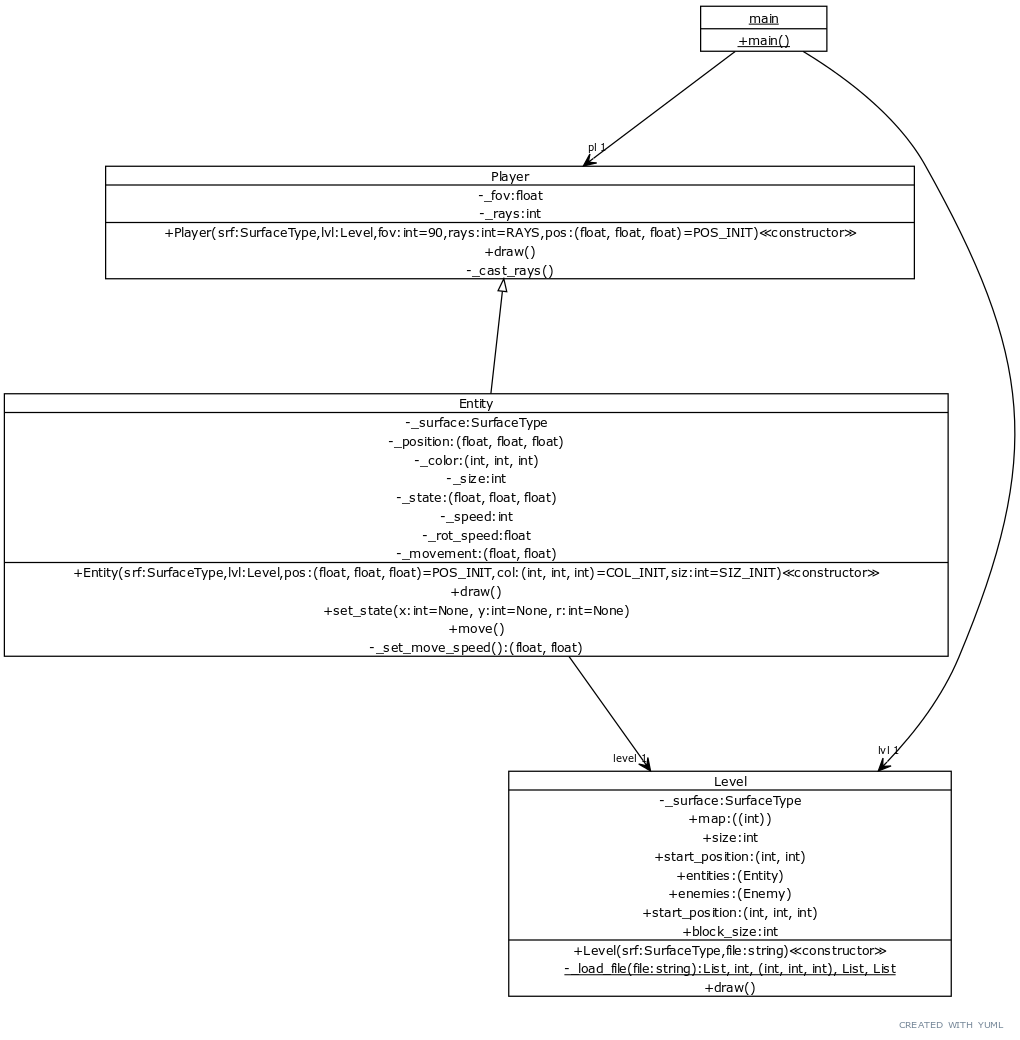
\includegraphics[scale=0.35]{./img/yuml1}

\newpage

\section{Steuerung}

\subsection{Command-Line Argumente}

\begin{itemize}
	\item \verb|-h --help| zeigt die CLI Argumente und beendet das Programm.
	\item \verb|-l --level| lädt das angegebene Level oder die angegebene Level Datei.
	\item \verb|--fov| ändert den Blickwinkel (angegeben in Grad) Standartwert ist 90°.
	\item \verb|--rays| ändert die horizontale Auflösung (Anzahl der gesendeten Strahlen) Standartwert ist 90. Höhere Werte können die Leistung beeinträchtigen.
\end{itemize}

\subsection{Levelerstellung}
Level werden im JSON-Format gespeichert.
\begin{itemize}
	\item \verb|"map": [[int]]| Die Map: 1 entspricht einer Wand, 0 Leerraum. Die Map muss quadratisch sein (ansonsten crasht das Programm)
	\item \verb|"size": int| Die Größe der Map. Muss dem tatsächlichen Wert entsprechen.
	\item \verb|"start_pos": [x: int, y: int, r: int]| Die Startposition des Spielers. X und y sind Werte zwischen 0 und 512, sie geben die Position in Pixeln an. R ist zwischen 0 und 360 und ist die Drehung in Grad.
	\item \verb|""entities": [], "enemies": []| Enthalten aktuell keine Werte und werden für zukünftigen Gebrauch freigehalten.
	
\end{itemize}

\subsection{Bewegung}

\subsubsection{Translation (Laufen)}
\begin{itemize}
\item Vorwärts: `W'
\item Links: `A'
\item Rückwärts: `S'
\item Rechts: `D'
\end{itemize}

\subsubsection{Rotation}
\begin{itemize}
\item Links: linke Pfeiltaste ($\leftarrow$)
\item Rechts: rechte Pfeiltaste ($\rightarrow$)
\end{itemize}

\subsection{UI}
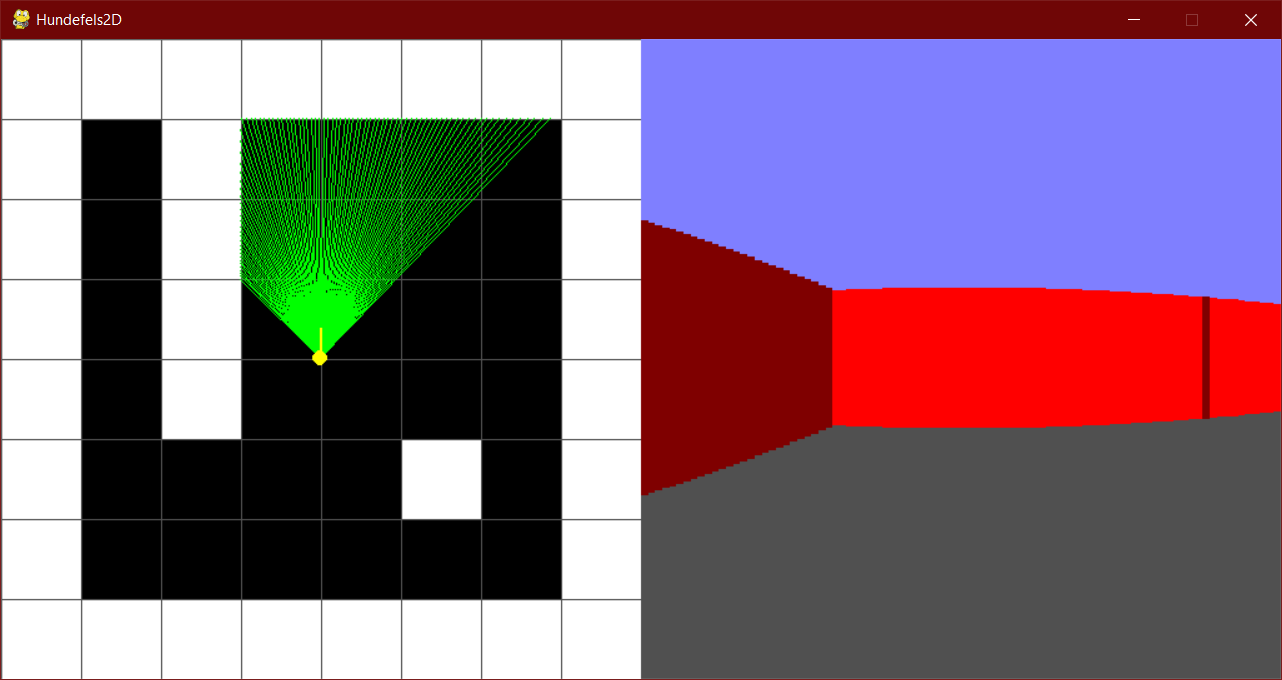
\includegraphics[scale=1.18]{./img/ui}

\newpage

\begin{flushleft}
\begin{thebibliography}{99}
\bibitem{rcp} 3DSage: ~ ``Make Your Own Raycaster Part 1'' ~ https://youtu.be/gYRrGTC7GtA\\ Quellcode verfügbar unter https://github.com/3DSage/OpenGL-Raycaster\_v1
\bibitem{pygame} Pygame tutorial: 	
\end{thebibliography}
\end{flushleft}

\end{document}